\documentclass[12pt]{article}
\usepackage[left=1cm, right=1cm, top=2cm,bottom=1.5cm]{geometry} 

\usepackage[parfill]{parskip}
\usepackage[utf8]{inputenc}
\usepackage[T2A]{fontenc}
\usepackage[russian]{babel}
\usepackage{enumitem}
\usepackage[normalem]{ulem}
\usepackage{amsfonts, amsmath, amsthm, amssymb, mathtools}

\usepackage{fancyhdr}
\pagestyle{fancy}
\renewcommand{\headrulewidth}{1.5pt}
\renewcommand{\footrulewidth}{1pt}

\usepackage{graphicx}
\usepackage[figurename=Рис.]{caption}
\usepackage{subcaption}
\usepackage{float}

%%Наименование папки откуда забирать изображения
\graphicspath{ {./images/} }

%%Изменение формата для ввода доказательства
\renewcommand{\proofname}{$\square$  \nopunct}
\renewcommand\qedsymbol{$\blacksquare$}

\addto\captionsrussian{%
	\renewcommand{\proofname}{$\square$ \nopunct}%
}
%% Римские цифры
\newcommand{\RN}[1]{%
	\textup{\uppercase\expandafter{\romannumeral#1}}%
}


\theoremstyle{definition}
\newtheorem{defn}{Опр:}
\newtheorem{rem}{Rm:}
\newtheorem{prop}{Утв.}
\newtheorem{exrc}{Упр.}
\newtheorem{lemma}{Лемма}
\newtheorem{theorem}{Теорема}
\newtheorem{corollary}{Следствие}

\newenvironment{cusdefn}[1]
{\renewcommand\thedefn{#1}\defn}
{\enddefn}



\DeclareRobustCommand{\divby}{%
	\mathrel{\text{\vbox{\baselineskip.65ex\lineskiplimit0pt\hbox{.}\hbox{.}\hbox{.}}}}%
}
\DeclareMathSymbol{\shortminus}{\mathbin}{AMSa}{"39}

\newcommand{\smallerrel}[1]{\mathrel{\mathpalette\smallerrelaux{#1}}}
\newcommand{\smallerrelaux}[2]{\raisebox{.1ex}{\scalebox{.75}{$#1#2$}}}

\newcommand{\smallin}{\smallerrel{\in}}
\newcommand{\smallnotin}{\smallerrel{\notin}}

\newcommand*{\medcap}{\mathbin{\scalebox{1.25}{\ensuremath{\cap}}}}%
\newcommand*{\medcup}{\mathbin{\scalebox{1.25}{\ensuremath{\cup}}}}%

\begin{document}
\lhead{Математический анализ - I}
\chead{Шапошников С.В.}
\rhead{Лекция - 18}

\subsection*{Структура множества точек разрыва}

$f$ - ограничена и определена на $\mathbb{R}$. Мы ввели понятия колебания и колебания функции в точке $a$:
$$\omega(f,E) = \sup\limits_{x,y \in E}|f(x) - f(y)|, \, \omega(f,a) = \lim\limits_{\delta \to 0+} \omega(f,\mathcal{U}_\delta(a))$$ 

\begin{prop}
	$f$ непрерывна в точке $a \Leftrightarrow \omega(f,a) = 0$.
\end{prop}	

\begin{corollary}
	Множество точек разрыва $ = \bigcup\limits_{n}\{\,a \colon \omega(f,a) \geq \frac{1}{n} \,\}$.
\end{corollary}

\begin{prop}
	Множество $\bigcup\limits_{n}\{\,a \colon \omega(f,a) \geq \frac{1}{n} \,\}$ - замкнуто.
\end{prop}
\begin{proof}
	Покажем, что дополнение - открыто. 
	
	Пусть $b \in \mathbb{R}\setminus\{\,a \colon \omega(f,a) \geq \frac{1}{n} \,\} = \{\,a \colon \omega(f,a) < \frac{1}{n} \,\} \Rightarrow$ надо показать, что $b$ принадлежит этому множеству с некоторой окрестностью. Знаем, что $\omega(f,b) <\frac{1}{n} \Rightarrow \lim\limits_{\delta \to 0+} \omega(f,\mathcal{U}_\delta(b)) < \frac{1}{n}$. По теореме отделимости при значениях $\delta$ близких к нулю, значения функции $\omega(f,\mathcal{U}_\delta(b)) < \frac{1}{n}$.
	
	Рассмотрим по определению: $\forall \varepsilon > 0, \, \exists \, \hat{\delta} >0 \colon \forall \delta \in (0, \hat{\delta}) \Rightarrow |\omega(f,\mathcal{U}_\delta(b)) - \omega(f,b)| < \varepsilon \Rightarrow$\\ $\Rightarrow \omega(f,\mathcal{U}_\delta(b)) < \omega(f,b) + \varepsilon$. Возьмем $\varepsilon = \frac{1}{n} - \omega(f,b) > 0 \Rightarrow$ 
	$$\omega(f,\mathcal{U}_\delta(b)) < \frac{1}{n} -  \omega(f,b) + \omega(f,b) = \frac{1}{n}$$
	Таким образом, $\exists \, \delta >0 \colon \omega(f,\mathcal{U}_\delta(b)) <  \frac{1}{n}$. 
	
	Возьмем точку $c$ из этого интервала $\mathcal{U}_\delta(b)$ и возьмем окрестность вокруг этой точки: $\mathcal{U}_\gamma (c)$ так, чтобы $\mathcal{U}_\gamma (c) \subset \mathcal{U}_\delta(b)$.
	
	\begin{figure}[H]
		\centering
		\includegraphics[width=0.35\textwidth]{18_1.eps}
		\caption{Колебания функции на интервале $\omega(f,\mathcal{U}_\gamma(c)) \leq \omega(f,\mathcal{U}_\delta(b))$.}
		\label{18_1}
	\end{figure}

	Точная верхняя грань на большем множестве не меньше, чем точная верхняя грань на меньшем $\Rightarrow \omega(f,\mathcal{U}_\gamma(c)) \leq \omega(f,\mathcal{U}_\delta(b)) < \frac{1}{n} \Rightarrow \lim\limits_{\gamma \to 0+} \omega(f,\mathcal{U}_\gamma(c)) = \omega(f,c) < \frac{1}{n}$ поскольку величины $\omega(f,\mathcal{U}_\gamma(c))$ убывают при стремлении $\gamma$ к нулю. Следовательно интервал $(b - \delta, b + \delta) \subset \mathbb{R}\setminus\{\,a \colon \omega(f,a) \geq \frac{1}{n} \,\} \Rightarrow$ дополнение открыто $\Rightarrow$ исходное множество замкнуто.
\end{proof}

Теорема выше говорит о том, что множество точек разрыва $f$ - это объединение не более чем счетного набора замкнутых множеств.

\textbf{Пример}: множество иррациональных чисел не является множеством точек разрыва.

\newpage

\section*{Глобальные свойства непрерывных функций}

\begin{defn}
	Функция $f$ \uwave{непрерывна на множестве} $D$, если функция $f$ непрерывна в каждой точке $D$ по множеству $D$.
\end{defn}

\subsection*{Первая теорема Вейрштрасса}
	
\begin{theorem}\textbf{(Первая теорема Вейрштрасса)}
	Если $f$ непрерывна на компакте $K$, то $f$ ограниченна на $K$, то есть $$\exists \, C > 0 \colon |f(x)| \leq C, \, \forall x \in K$$
\end{theorem}

\begin{proof}\hfill\\
	\textbf{(\RN{1}) способ:} (От противного) Пусть $\forall n, \, \exists \, x_n \in K \colon |f(x_n)| > n \Rightarrow$ получили последовательность по которой $|f(x_n)|$ уходит в бесконечность. Так как $K$ - компакт, то $\exists \, x_{n_k} \colon x_{n_k} \to x_0 \in K \Rightarrow$ из-за непрерывности $f \Rightarrow f(x_{n_k}) \to f(x_0)$, то есть, последовательность сходится к $f(x_0)$. 
	
	Но $|f(x_{n_k})| > n_k \to \infty$ что невозможно, так как если последовательность сходится, то она ограниченна $\Rightarrow$ противоречие.
	
	\textbf{(\RN{2}) способ:} $\forall a \in K, \, f$ - непрерывна в точке $a \Rightarrow \exists \, C_a >0 \wedge \mathcal{U}(a) \colon |f(x)|\leq C_a, \, \forall x \in \mathcal{U}(a)$. Заметим, что $K \subset \bigcup\limits_{a \in K} \mathcal{U}(a) \Rightarrow$ по определению компакта $\exists \, \mathcal{U}(a_1), \dotsc, \mathcal{U}(a_N) \colon K \subset \mathcal{U}(a_1) \cup \dotsc \cup \mathcal{U}(a_N)$. Тогда 
	$$C = \max\{C_{a_1},\dotsc, C_{a_N}\} \Rightarrow |f(x)| \leq C, \, \forall x \in K$$
	таким образом, $f$ ограниченна на $K$.
\end{proof}

\begin{rem}
	В данной теореме невозможно отказаться от компактности.
\end{rem}

\textbf{Пример}: $f(x) = \dfrac{1}{x}, \, x \in (0,1)$ - непрерывна, но не явлется ограниченной $\Rightarrow$ теорема не верна.

\begin{figure}[H]
	\centering
	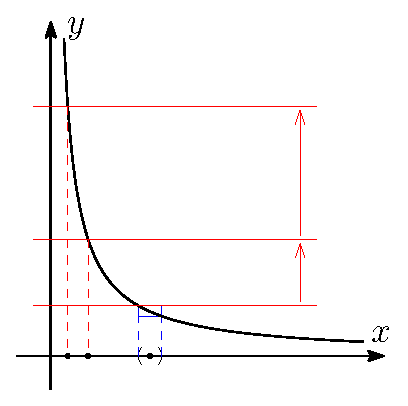
\includegraphics[width=0.3\textwidth]{18_2.eps}
	\caption{При приближении к $0$, у функции $\frac{1}{x}$ ограничивающая константа будет расти.}
	\label{18_2}
\end{figure}

\textbf{Пример}: $f(x) = \frac{1}{x}, \, x\neq 0 \wedge f(0) = 0, \, x \in [0,1]$ - множество является компактом, но функция разрывна в точке $0 \Rightarrow$ теорема не верна.

\subsection*{Вторая теорема Вейрштрасса}

\begin{theorem}\textbf{(Вторая теорема Вейрштрасса)}
	Если $f$ непрерывна на компакте $K$, то она принимает свои наибольшие и наименьшие значения на нем, то есть $$\exists \, x_m, x_M \in K \colon f(x_m) = \inf\limits_{x \in K} f(x), \, f(x_M) = \sup\limits_{x \in K} f(x)$$
\end{theorem}

\begin{rem}
	Нарушение любого из условий также влечет нарушение теоремы.
\end{rem}

\begin{figure}[H]
	\begin{subfigure}[b]{0.5\textwidth}
		\centering
		\includegraphics[width=0.6\textwidth]{18_3.eps}
		\caption{Непрерывная функция $y = x$ на интервале.}
		\label{18_3}
	\end{subfigure}%
	\begin{subfigure}[b]{0.5\textwidth}
		\centering
		\includegraphics[width=0.6\textwidth]{18_4.eps}
		\caption{Функция разрывна на компакте.}
		\label{18_4}
	\end{subfigure}
	\caption{Примеры нарушения условий теоремы Вейрштрасса.}
\end{figure}

\begin{proof}\hfill\\
	\textbf{(\RN{1}) способ:} $\forall n, \, \inf\limits_{x \in K} f(x) + \frac{1}{n}$ - не нижняя грань $\Rightarrow \exists \, x_n \in K \colon f(x_n) < \inf\limits_{x \in K} f(x) + \frac{1}{n} \Rightarrow$ получили последовательность точек компакта. Так как $K$ - компакт, то $\exists \, x_{n_k} \to x_0 \in K$. Для этой подпоследовательности выполнено 
	$$ \inf\limits_{x \in K}  f(x) \leq f(x_{n_k}) < \inf\limits_{x \in K} f(x) + \frac{1}{n_k}$$ 
	Пусть $k \to \infty \Rightarrow$ так как $f$ - непрерывна на компакте, то 
	$$f(x_{n_k}) \to f(x_0) \Rightarrow \inf\limits_{x \in K}  f(x) \leq f(x_0) \leq \inf\limits_{x \in K} f(x) \Rightarrow f(x_0) = \inf\limits_{x \in K} f(x) $$
	Аналогично для точной верхней грани.
	
	\textbf{(\RN{2}) способ:} (От противного) $\forall x \in K, \, f(x) > \inf\limits_{K}f(x)$. Рассмотрим новую функцию 
	$$g(x) = \dfrac{1}{f(x) - \inf\limits_{K} f(x)}$$
	По условию $f(x) - \inf\limits_{K}f(x) \neq 0, \, \forall x \in K$ - непрерывная функцию не обращающаяся в 0 на компакте $K \Rightarrow$ \\
	$\Rightarrow g(x)$ - тоже непрерывная функция на компакте $K$. По первой теореме Вейрштрасса, непрерывная на компакте функция - ограниченна $\Rightarrow \exists \, C>0 \colon g(x) < C, \, \forall x \in K \Rightarrow$
	$$\dfrac{1}{f(x) - \inf\limits_{K} f(x)} < C \Rightarrow \frac{1}{C} <  f(x) - \inf\limits_{K} f(x) \Rightarrow  \frac{1}{C} + \inf\limits_{K}{f(x)} <  f(x), \, \forall x \in K$$  
	Таким образом, получаем, что $\frac{1}{C} + \inf\limits_{K}{f(x)}$ - нижняя грань, но это невозможно, так как $\inf\limits_{K}{f(x)}$ - точная нижняя грань $\Rightarrow$ противоречие.
\end{proof}

\subsection*{Теорема Коши о промежуточном значении}
	
\begin{theorem}\textbf{(Коши)}
	Если $f$ непрерывна на отрезке $[a,b]$ и $f(a)f(b) < 0$ (на концах значения разных знаков), то $\exists \, c \in [a,b] \colon f(c) = 0$.
\end{theorem}

\begin{figure}[H]
	\centering
	\includegraphics[width=0.3\textwidth]{18_5.eps}
	\caption{Функция, непрерывная на отрезка $[a,b]$ с разными значениями на концах.}
	\label{18_5}
\end{figure}

\begin{proof}\hfill\\
	\textbf{(\RN{1}) способ:} Делим отрезок $[a,b]$ пополам, если $f(\frac{a+b}{2}) = 0$, то $c = \frac{a+b}{2}$. Если $f(\frac{a+b}{2}) \neq 0$, то 
	$$f(\tfrac{a+b}{2})f(a) < 0 \vee f(\tfrac{a+b}{2})f(b) < 0$$ Пусть $[a_1,b_1]$ - та половина на концах которой разные знаки, $b_1 - a_1 = \frac{b-a}{2}$.

	\begin{figure}[H]
		\centering
		\includegraphics[width=0.3\textwidth]{18_6.eps}
		\caption{Поиск отрезка со значениями разных знаков на концах.}
		\label{18_6}
	\end{figure}
	
	Повторяем рассуждения для $[a_1, b_1]$: либо $f(\frac{a_1+b_1}{2}) = 0 \Rightarrow c = \frac{a_1+b_1}{2}$, либо $f(\frac{a_1+b_1}{2}) \neq 0$ и $[a_2, b_2]$ - та половина $[a_1,b_1]$, на концах которой $f$ принимает значения разных знаков. И так далее.
	
	В итоге, либо на каком-то шаге найдена точка $c$, либо построена последовательность вложенных отрезков $[a_1,b_1] \supset [a_2,b_2] \supset \dotsc \supset [a_n, b_n] \supset \dotsc$ такая, что их длины $b_n - a_n = \frac{b-a}{2^n} \to 0$ и $f(a_n) f(b_n) <0$. 
	
	По теореме о вложенных отрезках $\exists \, c \in \bigcap\limits_n [a_n, b_n]$. Так как $c$ лежит внутри отрезков, то $$|c - a_n| \leq \tfrac{b-a}{2^n} \wedge |c - b_n| \leq \tfrac{b-a}{2^n} \Rightarrow a_n \to c \wedge b_n \to c$$ 
	Так как $f$ - непрерывна в точке $c$, то 
	$$f(a_n) \to f(c) \wedge f(b_n) \to f(c) \Rightarrow f(c)^2 = \lim\limits_{n\to \infty} f(a_n)f(b_n) \leq 0 \Rightarrow f(c) = 0$$
	
	\textbf{(\RN{2}) способ:} (От противного) Пусть $f(a) < 0, \, f(b) > 0$ и $f(x) \neq 0$ на отрезке $[a,b]$. Рассмотрим множество $F^- = \{\,x \in [a,b] \colon f(x) \leq 0 \,\}$ и множество $F^+ = \{\,x \in [a,b] \colon f(x) \geq 0 \,\}$. 
	Очевидно, что 
	\begin{enumerate}[label={\arabic*)}]
		\item $F^- \cap F^+ = \varnothing, \, F^- \cup F^+ = [a,b]$;
		\item $a \in F^-, \, b \in F^+$, то есть эти множества не пусты;
		\item $F^- \wedge F^+$ - замкнуты;
	\end{enumerate}

	Доказав $3)$, мы представим отрезок в виде двух непересекающихся и непустых замкнутых множеств. Добавим к одному из них $(-\infty, a]$, а к другому $[b, +\infty) \Rightarrow$ получится, что всю числовую прямую представили в виде объединения двух непересекающихся, непустых, замкнутых множеств $\Rightarrow$ противоречие.
	
	Пусть $x_n \in F^- \wedge x_n \to x_0 \Rightarrow f(x_n) \leq 0$, из-за непрерывности $f(x_n) \to f(x_0)\Rightarrow f(x_0) \leq 0 \wedge x_0 \in F \Rightarrow$ это множество замкнуто. Аналогично для $F^+$.
	
	Вся числовая прямая представляется, как $\mathbb{R} = \big((-\infty,a] \cup F^- \big) \cup \big( F^+ \cup  [b,+\infty)\big)$. Эти два множества - не пересекаются, так как $F^- \cap F^+ = \varnothing$ и $a \in F^-, \, b \in F^+$. Также эти множества не пустые и замкнутые, что невозможно $\Rightarrow$ противоречие со связностью прямой (числовую прямую нельзя представить в виде объединения двух замкнутых множеств).
\end{proof}	

\begin{rem}
	Замкнутость множества нулей непрерывной функции доказывается аналогично доказательству замкнутости множеств $F^-$ и $F^+$.
\end{rem}

\begin{exrc}
	Доказать, что всякое замкнутое множество является множеством нулей некоторой непрерывной функции.
\end{exrc}

\begin{corollary}\textbf{(Теорема о промежуточном значении)}
	Пусть $f$ непрерывна на отрезке $[a,b]$ и \\
	$A = f(a), \, B = f(b)$. Тогда $\forall C \colon A \leq C \leq B, \, \exists \, c\in [a,b] \colon f(c) = C$.
\end{corollary}

\begin{proof}
	Рассмотрим функцию $g(x) = f(x) - C$. Если $C \neq A \wedge C \neq B \Rightarrow g(a)g(b) = (A - C)(B - C) < 0 \Rightarrow$ по предыдущей теореме $\exists \, c \in [a,b] \colon g(c) = 0 \Leftrightarrow f(c) - C = 0 \Leftrightarrow f(c) = C$.
\end{proof}

\textbf{Пример}: $x^3 + ax^2 + bx + c =0$ - обязательно $\exists$ корень $\in \mathbb{R}$. 
$f(x) = x^3\big(1 + \tfrac{a}{x} + \tfrac{b}{x^2} + \tfrac{c}{x^3}\big) \Rightarrow \tfrac{a}{x} + \tfrac{b}{x^2} + \tfrac{c}{x^3} \to 0$ при больших $x \Rightarrow$ знак определяется по $x^3$. Возьмем отрезок с большим отрицательным значением на левом конце и большим положительным значением на правом, $x^3$ будет разных знаков на этих концах $\Rightarrow$ по теореме о промежуточном значении существует точка в которой функция обращается в 0.

\end{document}